\chapter{Wave Stage} \label{ch:wave_preproc}
Earth Observation techniques have been experiencing a growth both in terms of quality and quantity, which means that the amount of data produced have also increased drastically. In addition, remote sensing is usually carried out by satellites with low storage capacity and limited bandwidth \parencite{SANDAU20101}, so clearly data compression is key in this situation.

Some satellites collect \acrshort{rf} data, either from ground or air sources (e.g. vessels, airplanes or industrial activity in general), as well as from other satellites. Between the vast amount of remote sensing techniques we find Radio Occultation \parencite{RO-GNSS}, which uses low orbit satellites to detect the changes produced by the atmosphere in a radio signal emitted by a \acrshort{gnss} satellite. \acrshort{ro} data is mainly used as a weather forecasting tool.

\begin{figure}[h!]
	\begin{center}
		\begin{tabular}{ @{} c @{} }
			\includegraphics[scale=0.44]{images/ro_schematic.jpg}\\
			\imagesource{Wikipedia user MPRennie, CC BY-SA 3.0, via Wikimedia Commons.}
		\end{tabular}
	\end{center}
	\vspace*{-0.7em}
	\caption{Illustration of radio occultation (RO).}
	\label{fig:ro_schematic}
\end{figure}

This chapter is part of a DAPCOM Data Services strategic project focused on developing a new \acrshort{fapec} stage intended to compress data collected by satellites. The algorithm will be tested over \acrshort{iq} sample files and other formats structured in two channels, for instance, stereo audio. The proposed solution will be compared with the well-known \acrshort{flac} coding technique.

\section{Introduction to IQ data}

In the introduction of this chapter we stated that the present stage will be focused on \acrshort{iq} data, that is, the discrete time samples of a \acrshort{rf} \acrshort{iq} signal.

From Communication Theory we know that any pass-band signal $s(t)$ can be expressed as:
\begin{equation}
s(t) = i_s(t) \cdot \cos(2\pi f_0 t) - q_s(t) \cdot \sin(2\pi f_0 t)
\end{equation}

Where:
\begin{description}
	\item $i_s(t) \equiv$ In-phase component of the RF signal.
	\item $q_s(t) \equiv$ Quadrature component of the RF signal.
	\item $f_0 \equiv$ Carrier frequency of the RF signal.
\end{description}

For simplicity, we may work with the equivalent base-band signal $b_s(t)$:
\begin{equation}
	b_s(t) = i_s(t) + j q_s(t)
\end{equation}

Hence, the data to be compressed are the discrete time samples of the signals $i_s(t)$ and $q_s(t)$. In other words, our aim is to compress time series data separated in two channels.

For further information on \acrshort{iq} signals the reader may check references \parencite{IQintro}, \parencite{carlson2010communication} and \parencite{ICOM}.

\section{Motivation and applications of Wave} \label{sec:wave_motivation}
We shall provide a justification on why we can use both \acrshort{iq} and audio files to test Wave and why we can compare it with the \acrshort{flac} standard.

On the first hand, as we will see shortly, both \acrshort{flac} and Wave implement the same preprocessing stage: a classical linear predictor. This decorrelation stage is followed by a Rice-Golomb entropy coder (see section \ref{golomb-coding}) in \acrshort{flac} and by the \acrshort{fapec} entropy coder in Wave.

On the other hand, \acrshort{iq} data and stereo audio have the same structure: time series separated in two channels (notice that samples distribution may not be the same). In fact, most \acrshort{sdr} records are stored as \acrshort{wav} files, a well known audio format.

Additionally, in literature we may find papers about \acrshort{iq} data compression that make use of the \acrshort{flac} algorithm, for instance \parencite{IQFlac}.

To conclude, there are clear similarities between the two proposed algorithms and also between the proposed data formats. Hence, from a qualitative point of view, comparing Wave and \acrshort{flac} with a dataset of \acrshort{iq} data and stereo audio files is a logical choice.

\section{Design}
In this section we will design the algorithm intended to decorrelate audio and \acrshort{iq} data. The structure of the section will be the following: first we will state the specific requirements for the stage. Then, according to these and to the data structure described above, an algorithm will be proposed.

\subsection{Requirements and specifications}
Besides the general requirements and specifications for \acrshort{fapec} stages described in section \ref{sec:fapec_reqs}, Wave must also fulfill:
\begin{enumerate}
	\item Compression ratio must be at least an 80\% of \acrshort{flac}'s.
	\item Compression speed must be better than \acrshort{flac}'s.
	\item It shall work for an arbitrary number of channels.
	\item It shall work for 8-bit and 16-bit samples.
\end{enumerate}

\subsection{Algorithm design}
In section \ref{sec:wave_motivation} we justified why \acrshort{flac} should have a good performance with \acrshort{iq} data. Taking this into account, the proposed algorithm should have a structure similar to \acrshort{flac}'s but using \acrshort{fapec} as the entropy coder. This should translate into a compressor faster than \acrshort{flac} and with a similar compression ratio.

From the \acrshort{flac} format specifications we know that its preprocessing stage is based in a linear predictor \parencite{FLAC}. Therefore, our goal is to implement a predictor which, given an input sequence $x(n)$, predicts future samples following the model
\begin{equation} \label{eq:prediction_x}
\hat{x}(n) = \sum_{i=1}^{Q} h_i x(n-i)
\end{equation}
where $\hat{x}(n)$ is the predicted sequence, $x(n-i)$ the previous observed samples, $h_i$ the filter coefficients and $Q$ the filter order.

From filter theory \parencite{PSAVC} we know that the coefficients $h_i$ are given by
\begin{equation} \label{eq:normal_eqs_matrix}
\mathbf{R}_x \mathbf{h} = \mathbf{r}_x
\end{equation}
where $\mathbf{R}_x$ is a $Q \times Q$ Toeplitz matrix with elements $r_{ij} = r_x(|i-j|),\hspace{0.5em} 0 \leq i,j < Q$, $\mathbf{r}_x$ the correlation vector with $r_j = r_x(j),\hspace{0.5em} 0 < j \leq Q$ and $\mathbf{h}$ the filter coefficients.

Equation \ref{eq:normal_eqs_matrix} can also be expressed with scalar notation as:
\begin{equation} \label{eq:normal_equations}
r_x(j) = \sum_{i=1}^{Q} h_i r_x(|i-j|) ,\hspace{0.5em} 0 < j \leq Q
\end{equation}
where $r_x(j)$ is the lag $j$ of the autocorrelation of $x(n)$.

In order to obtain the filter coefficients $h_i$ we need to solve the previous system. In this case, using Gauss-Jordan elimination is not desirable as it has a complexity of $O(Q^3)$. However, there exist algorithms such as the Levinson-Durbin recursion \parencite{LevinsonDurbin} which, taking advantage of the Toeplitz structure of $\mathbf{R}_x$, reduce the computational complexity to $O(Q^2)$.

Equation \ref{eq:normal_eqs_matrix} is obtained from a statistical approach to the problem, assuming that the sequence $x(n)$ is \acrshort{wss}. However, in our case $x(n)$ is a deterministic finite sequence from an unknown origin. For this reason, we need to split $x(n)$ in subsequences $x_N(n)$ of length $N$ where assuming stationarity is reasonable. For each of these subsequences $x_N(n)$, the filter coefficients $h_i$ are assumed to be independent (i.e. they are reset at the beginning of each subsequence). In this scenario, the autocorrelation lags for each subsequence would be given by the short-term autocorrelation function:
\begin{equation}
r_x(i) = \sum_{m=0}^{N-1-i} x_N(m) x_N(m+i) ,\hspace{0.5em} i \geq 0
\end{equation}

It is important to remark that given the unknown character of the input data, $N$ is a custom parameter that the user may choose when setting up the compressor.

However, for computational purposes, we will not use all the $N$ samples of $x_N(n)$. Instead, we will set a training length $T \leq N$ and the autocorrelation lags will be calculated as follows:
\begin{equation}
	r_x(i) = \sum_{m=0}^{T-1-i} x_N(m) x_N(m+i) ,\hspace{0.5em} i \geq 0
\end{equation}

If lossy is enabled, samples will be divided and then floored just before this step. It is important to notice that lossy must be applied to samples instead of prediction errors to avoid accumulating quantization errors.

To sum up, the proposed algorithm consists in splitting $x(n)$ in sequences of size $N$ for which the autocorrelation will be computed using $T$ samples. Then, the filter coefficients $h_i$ will be computed using the Levinson-Durbin algorithm and they will be sent to the entropy coder together with the prediction errors given by:
\begin{equation}
e(n) = x(n) - \hat{x}(n)
\end{equation}

We should point out that recovering samples in decompression is as easy as calculating $\hat{x}(n)$ with equation \ref{eq:prediction_x} and then adding it to the prediction error for that sample (remember that we coded the prediction errors and the coefficients). Taking this into account, it is obvious that decompression will be much faster than compression.

In general, the previous algorithm will be applied independently in each channel, but the user may enable channel coupling and then the coefficients from the first channel will be reused in the others.

In figure \ref{fig:wave_flowchart} we include a flowchart for the proposed algorithm, where \textit{Settings} are the number of bits per sample, a boolean to enable or disable channel coupling, the level of losses, the number of channels, the period length $N$, the training length $T$ and the filter order $Q$.

\begin{figure}[h!]
	\begin{center}
		\scalebox{.71}{\begin{tikzpicture}[
        every node/.style={draw,minimum width=3cm,minimum height=1cm},
        every text node part/.style={align=center},
         node distance=2.6cm and 3.8cm, on grid,
        >={Stealth[length=2mm]},
        inici/.style={rounded rectangle,minimum height=1cm,fill=ForestGreen!20},
        parametres/.style={
            trapezium,
            shape border rotate=90,
            trapezium left angle=90, 
            trapezium right angle=80,
            minimum width=1cm,
            fill=yellow!30,
        },
        entrada/.style={tape,minimum width=1.5cm,fill=violet!20},
        rectangle/.style={minimum width=3.0cm,fill=blue!10},
        decisio/.style={diamond,minimum height=1.7cm,aspect=1.6,fill=red!10},
        coordenada/.style={draw=none,minimum width=0},
        bool/.style={draw=none,minimum width=0,minimum height=0},
    ]
    \scriptsize
    % Dibuixo primer els nodes i després les fletxes. Hi ha diverses maneres de fer-ho
    \node[inici,minimum width=4cm] (start) {Start};
    \node[entrada] (input) at (-1.3,2) {Input file};
    \node[parametres] (settings) at (1,2) {Settings};
    \node[decisio,below=of start] (D1) {More periods?};
    \node[inici, below=of D1] (end) {End};
	\node[rectangle, right=of D1] (samples) {Extract samples};
	\node[decisio,below=of samples] (D2) {More channels?};
	\node[decisio,below=of D2] (D3) {Lossy?};
	\node[rectangle, right=of D3] (divide) {Divide samples};
	\node[decisio,below=of D3] (D4) {Coupling?};
	\node[decisio,right=of D4] (D5) {First channel?};
	\node[rectangle, below=of D4] (autocorr) {Find autocorrelation};
	\node[rectangle, below=of autocorr] (levinson) {Levinson-Durbin};
	\node[rectangle, below=of levinson] (estimations) {Find estimation errors};
	\node[rectangle, below=of estimations] (coder) {Entropy coder};

	% Dibuixo les fletxes
	\draw[->] (input) -- ++(0,-1.5);
    \draw[->] (settings) -- ++(0,-1.5);
	\draw[->] (start) -- node[coordenada,midway,name=P1] {} (D1);
	\draw[->] (D1) -- (end);
    \draw[->] (D1) -- (samples);
    \draw[->] (samples) -- node[coordenada,midway,name=P2] {} (D2);
    \draw[->] (D2) -- (D3);
	\draw[->] (D3) -- (divide);
	\draw[->] (D3) -- node[coordenada,midway,name=P3] {} (D4);
	\draw[->] (divide) |- (P3.center);
	\draw[->] (D4) -- (D5);
	\draw[->] (D4) -- node[coordenada,midway,name=P4] {} (autocorr);
	\draw[->] (D5) |- (P4.center);
	\draw[->] (autocorr) -- (levinson);
	\draw[->] (levinson) -- node[coordenada,midway,name=P5] {} (estimations);
	\draw[->] (D5.east) -- ++(0.8,0) |- (P5.center);
	\draw[->] (estimations) -- (coder);
	\draw[->] (coder.west) -- ++(-0.5,0) |- (P2.center);
	\draw[->] (D2.east) -- ++(0.85,0) |- (P1.center);

	% Ara els True/False escampats aquí i allí
    \node[bool,anchor=south west] at (D1.east) {True};
    \node[bool,anchor=north east] at (D1.south) {False};

    \node[bool,anchor=south west] at (D2.east) {False};
    \node[bool,anchor=north east] at (D2.south) {True};

    \node[bool,anchor=south west] at (D3.east) {True};
    \node[bool,anchor=north east] at (D3.south) {False};

    \node[bool,anchor=south west] at (D4.east) {True};
    \node[bool,anchor=north east] at (D4.south) {False};

    \node[bool,anchor=south west] at (D5.east) {False};
    \node[bool,anchor=north east] at (D5.south) {True};
\end{tikzpicture}}
	\end{center}
	\caption{Flowchart of the Wave preprocessing stage.}
	\label{fig:wave_flowchart}
\end{figure}

\section{Results}
The final step in the development of a new stage is evaluating it. To do that, we will use the metrics proposed in section \ref{sec:metrics}.

The results presented in this section have been obtained with the following settings:
\begin{itemize}
	\item Signed 16-bit samples.
	\item Filter order: $Q = 10$
	\item Period length: $N = 65536$
	\item Training length: $T = 65536$
	\item Number of channels: 2.
	\item No coupling.
	\item No losses.
\end{itemize}

Here we will include negentropies, ratios, execution times and Euclidean distances for all our dataset, but we will just show the histogram and the cumulative histogram for one file. The remaining ones can be found in appendix \ref{ch:wave_hists}.

We start our evaluation by showing the histogram (and cumulative histogram) of the song \textit{Formigues}, by Manel:

\begin{figure}[h!]
	\centering
	\begin{subfigure}{0.5\textwidth}
		\centering
		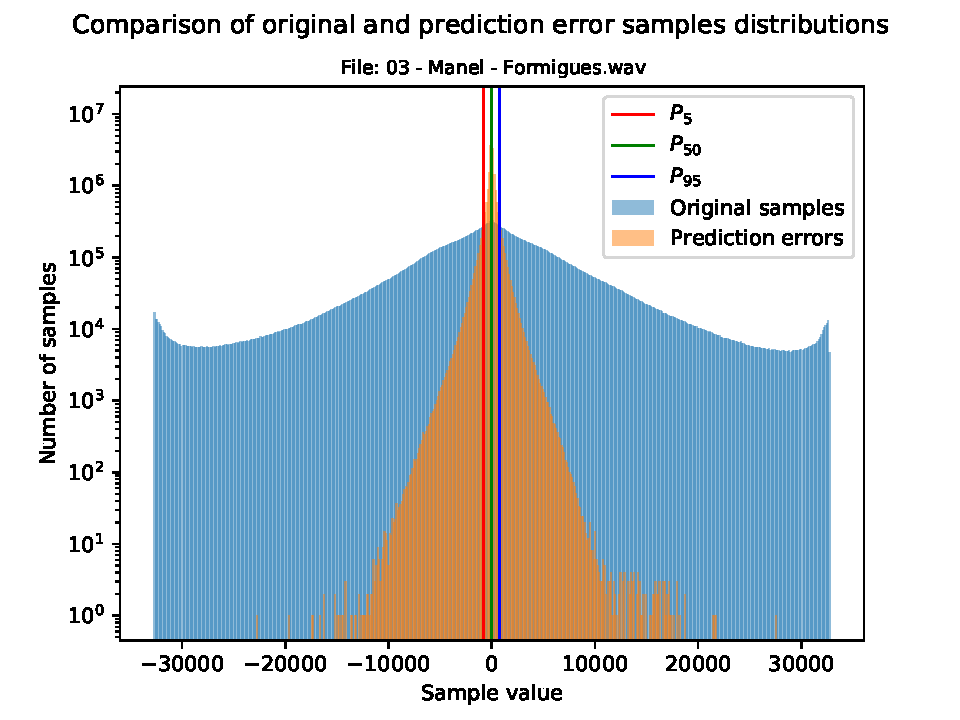
\includegraphics[width=\linewidth]{images/03 - Manel - Formigues.wav_hist.pdf}
		\caption{Histogram.}
		\label{fig:hist_formiques}
	\end{subfigure}%
	\begin{subfigure}{0.5\textwidth}
		\centering
		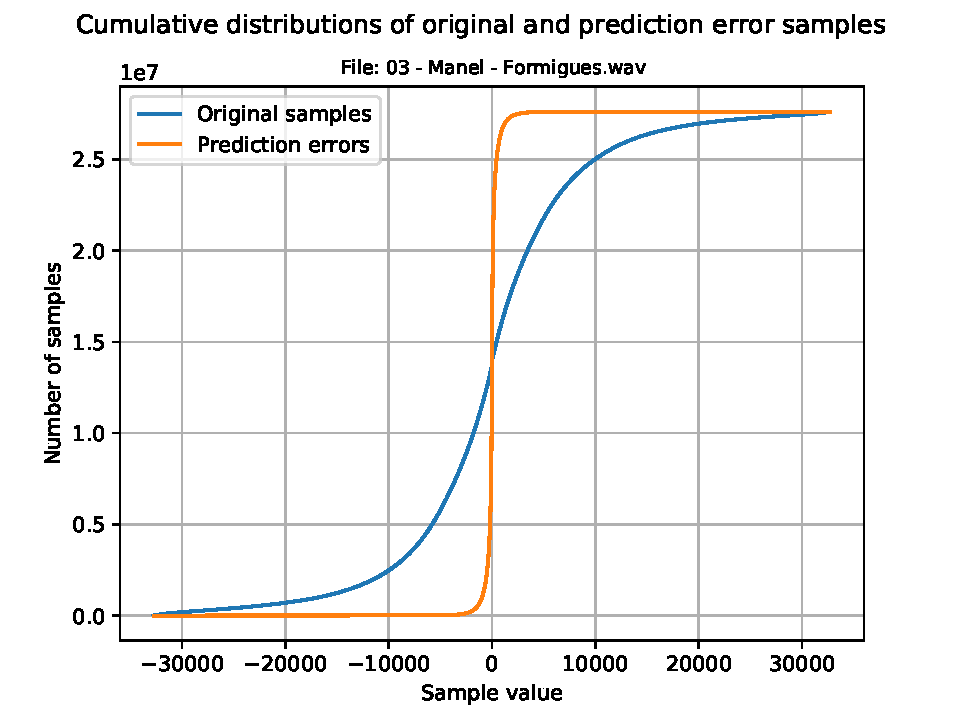
\includegraphics[width=\linewidth]{images/03 - Manel - Formigues.wav_hist_cum.pdf}
		\caption{Cumulative histogram.}
		\label{fig:cum_hists_formigues}
	\end{subfigure}
	\caption{Histograms of \textit{Formigues} by Manel.}
	\label{fig:formigues}
\end{figure}

We clearly see that histograms provide us a qualitative and visual way to identify the reduction of the dynamic range, but they are easy to manipulate with a simple division of the samples. Besides, we are also interested in quantifying this improvement. For this reason, we have estimated negentropy before and after the decorrelation process. Notice that an improvement of $\alpha$ times in negentropy does not imply that the compression ratio will be $\alpha$ times better.

As we can see in table \ref{tab:negentropies_wave}, negentropy of all files improves after applying the stage we have developed.

\begin{table}[h!]
\normalsize
\centering
\begin{tabular}{|
	>{\columncolor[HTML]{FFFFFF}}l |
	>{\columncolor[HTML]{FFFFFF}}c |
	>{\columncolor[HTML]{FFFFFF}}c |c|}
	\hline
	\multicolumn{1}{|c|}{\cellcolor[HTML]{9698ED}Filename} & \cellcolor[HTML]{9698ED}J(X) & \cellcolor[HTML]{9698ED}J(E) & \cellcolor[HTML]{9698ED}J(E)/J(X) \\ \hline
	03 - Manel - Formigues.wav                             & 0.0018                       & 0.0144                       & 8.0                               \\ \hline
	04 - Pink Floyd - Time.wav                             & 0.0004                       & 0.0238                       & 59.5                              \\ \hline
	06 - Manel - Els entusiasmats.wav                      & 0.0012                       & 0.0098                       & 8.2                               \\ \hline
	06 - Pink Floyd - Money.wav                            & 0.0009                       & 0.0090                       & 10                                \\ \hline
\end{tabular}
\caption{Negentropies of audio files before and after Wave.}
\label{tab:negentropies_wave}
\end{table}

Finally, we will compare compression ratio and time of \acrshort{fapec}, \acrshort{flac} and GZIP.

\begin{figure}[h!]
	\begin{center}
		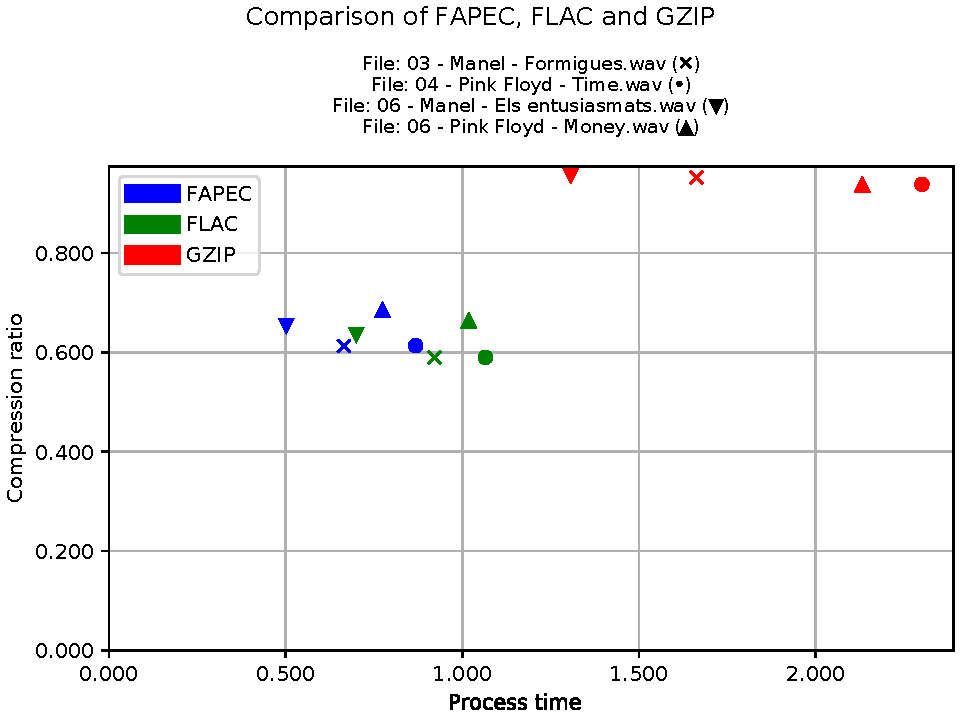
\includegraphics[scale=0.69]{images/2021-05-30T22:30:32.186296-results_wave.csv_comparison.pdf}
	\end{center}
	\caption{Comparison of audio compressors by time and ratio.}
	\label{fig:audio_compare}
\end{figure}

As we can see in figure \ref{fig:audio_compare}, \acrshort{flac} and \acrshort{fapec} have a similar performance, with the former having a better radio and the latter being faster. Applying our Euclidean distance criteria, we determine the \acrshort{fapec} behaves slightly better than \acrshort{flac} thanks to its speed. In table \ref{tab:audio_compare} we include the numerical values of the Euclidean distances.

\begin{table}[h!]
\normalsize
\centering
\begin{tabular}{|
	>{\columncolor[HTML]{FFFFFF}}l |
	>{\columncolor[HTML]{FFFFFF}}c |
	>{\columncolor[HTML]{FFFFFF}}c |c|}
	\hline
	\multicolumn{1}{|c|}{\cellcolor[HTML]{9698ED}Filename} & \cellcolor[HTML]{9698ED}FAPEC dist. & \cellcolor[HTML]{9698ED}FLAC dist. & \cellcolor[HTML]{9698ED}GZIP dist. \\ \hline
	03 - Manel - Formigues.wav                             & 0.9040                                 & 1.0938                                & 1.9161                                \\ \hline
	04 - Pink Floyd - Time.wav                             & 1.0630                                 & 1.2181                                & 2.4851                                \\ \hline
	06 - Manel - Els entusiasmats.wav                      & 0.8242                                 & 0.9453                                & 1.6197                                \\ \hline
	06 - Pink Floyd - Money.wav                            & 1.0333                                 & 1.2152                                & 2.3294                                \\ \hline
\end{tabular}
\caption{Wave Euclidean distances.}
\label{tab:audio_compare}
\end{table}

Finally, we want to present a brief code evaluation. The McCabe complexity of the stage is 31, smaller than the maximum value set in the specifications. Besides, in the worst scenario, the maximum occupied memory is 18.3 MB.

Our last remark is that all the requirements and specifications are fulfilled.
